\chapter{Conclusions} \label{chap:concl}

\minitoc

The field of \ac{DL} and audio has witnessed the emergence of generative \ac{AI} models for audio synthesis, a challenging and fascinating research topic. This thesis has investigated the evolution and evaluation of these models, with the main objectives of understanding the current state of the art and creating a novel model using a generative approach. To achieve these goals, this thesis has followed a comprehensive methodology that included conducting a literature review and developing and evaluating a generative \ac{AI} model for audio synthesis.

This chapter concludes the thesis by presenting the main results and contributions of the research. It also reflects on the research process and methodology, and suggests future directions for further research.

The first section, Section~\ref{sec:reflection-goals}, of this chapter provides an overview of the research goals that guided the investigation into the development and evaluation of generative \ac{AI} models for audio synthesis. Section~\ref{sec:reflection-process} reflects on the research process and methodology employed throughout the research, highlighting the strengths and limitations of the chosen approach, and discussing the challenges and lessons learned during the development of the \ac{AI} models. The third section, \ref{sec:future-directions}, outlines potential areas of future work that can help advance the field of generative \ac{AI} models for audio synthesis, addressing some of the open questions and limitations identified in the research.

\section{Overview of Research Goals} \label{sec:reflection-goals}

This section presents an overview of the research goals that directed the examination into the evolution and evaluation of generative \ac{AI} models for audio synthesis.

The two research goals can be summarized as follows: to understand the current state of the art in generative \ac{DL} and audio, and to create one of these models.

\subsection{Comprehensive Study of State-of-the-Art Deep Learning Architectures and Models for Audio Synthesis}

Throughout the thesis, a comprehensive study of the current state-of-the-art deep learning architectures for audio synthesis was conducted, including \acp{GAN}, \acp{VAE}, diffusion models, and other related architectures. This study included an in-depth analysis of the strengths, limitations, and potential applications of these architectures in the context of audio synthesis.

In addition, various models that use these deep learning architectures were examined, such as VALL-E, AudioGen, AudioLM, and others. Each model was thoroughly analyzed to understand their unique approaches, techniques, and contributions to audio synthesis. The results of this study provided valuable insights into the different models and their effectiveness in producing high-quality audio.

Extensive research was also conducted to examine previous algorithms used for sound processing, including techniques for augmentation, feature extraction, and other purposes. This research involved a thorough review of existing algorithms and their applicability to audio generative models. The insights gained from this research were used in the development of practical systems and contributed to the overall understanding of sound processing techniques in the context of generative AI models.

This work culminated in a thorough state-of-the-art chapter (Chapter~\ref{chap:sota}), which provides a comprehensive overview of current advances in deep learning architectures and models for audio synthesis. The chapter presents a detailed analysis of the studied architectures and models, highlighting their strengths, limitations, and potential applications.

In addition, the findings and insights from this research have been summarized in a review paper that has been submitted to a prestigious journal for peer review. This review paper aims to provide a comprehensive and up-to-date overview of the state of the art in deep learning architectures and models for audio synthesis. It is currently awaiting approval and publication in the journal.

\subsection{Developing End-to-End Systems for Sound Synthesis and Evaluation}

The goal of developing end-to-end systems for sound synthesis from text input has been partially achieved. While initial prototypes have been created, the results have not been satisfactory due to limitations in the available datasets and the lack of hyperparameter fine-tuning in the models. However, the potential for improvement is significant, and future work proposed in the conclusion suggests new models that could yield better results.

The goal of evaluating the ability of systems to generate sound from textual input remains an ongoing challenge. Finding and testing robust evaluation functions is a complex task that requires further research and dedicated effort. Due to time constraints, this objective has not been fully completed, and only a comparison using the loss function of \ac{GAN} has been performed. 

In summary, the research objectives outlined in this dissertation have been addressed to varying degrees. A comprehensive study of \ac{DL} architectures and prior sound processing algorithms has been conducted. The development of end-to-end systems for sound synthesis from text input has shown promising progress, while the evaluation of their accuracy remains an ongoing challenge. These achievements contribute to the existing knowledge and understanding of audio generative models and pave the way for future research and development in this area.

\section{Reflection on the Research Process} \label{sec:reflection-process}

Throughout this research, a comprehensive methodology was employed to ensure the successful achievement of the research objectives. The chosen methodology is presented in Section~\ref{sec:sol-approach} and involved conducting a thorough review of the state of the art while simultaneously initiating the writing process. This iterative and agile approach allowed for continuous refinement of ideas and incorporation of the latest developments in the field.

Reflecting on the effectiveness of the chosen methodology, it can be concluded that it successfully guided the research process. The methodology provided a structured framework for conducting the research and ensured that the objectives were addressed in a systematic and efficient manner. The challenges encountered during the research process were not related to the methodology itself, but rather to the complexity of the chosen research topic.

One challenge encountered during the research process was the sometimes tedious and frustrating nature of developing \ac{AI} models. Troubleshooting problems during training required additional time and effort, often requiring extended training periods to evaluate potential solutions. However, these challenges provided valuable lessons in patience, problem solving, and the importance of careful experimentation.


\section{Future Directions} \label{sec:future-directions}

The study and development of generative \ac{AI} models for audio synthesis have shown promising results in producing realistic and diverse audio output. However, there are still several avenues for further exploration and improvement. This section outlines potential areas of future work that can help advance the field of generative \ac{AI} models for audio synthesis.

\subsection{Exploring Novel Architectures}

The objective of this section is to recommend new frameworks that expand upon the groundwork established in this thesis. Developing these suggested frameworks is deferred to future research due to limited time and resources.

The proposed theoretical methods presented in this Section are motivated by the necessity of increasing the quality, diversity, and efficacy of the produced audio.

This section outlines the objectives, design principles, and possible applications of each suggested architecture. Furthermore, it discusses the methodological considerations and potential obstacles that may arise during their development and implementation.

It is essential to note that the proposed theoretical approaches presented here are intended to serve as a basis for future research. Researchers and practitioners are encouraged to explore, refine, and contribute to the advancement of generative \ac{AI} models for audio synthesis.

This section provides detailed explanations of each proposed architecture, including insights into its design principles, implementation considerations, and potential applications. This approach aims to stimulate further exploration and innovation in the field.

\subsubsection{VAMOS - Variable Audio Model for Sound Synthesis}

In the field of audio and sound processing, VAMOS (Variable Audio Model for Sound Synthesis) is a novel implementation inspired by the well-known DALL-E 2 framework (see Section~\ref{sec:dall-e-2}). While DALL-E 2's lies in its ability to generate images from textual descriptions, VAMOS extends this concept to the auditory domain, generating audio outputs based on corresponding textual inputs. This section describes the architecture, components, and underlying mechanisms that make up the VAMOS model.

Indeed, the VAMOS model goes beyond mere conceptualization, as its development was diligently initiated from the ground up. The foundation of this innovative model has been established through craftsmanship, with each component designed. The VAMOS architecture is available in open-source. Appendix~\ref{ann:vamos} shows and explains the significant code portions.

\paragraph{Model Composition}

VAMOS is comprised of four distinct yet interconnected models, each contributing to a comprehensive audio generation process. These models — CLAP, Text Encoder, Audio Encoder (ResNet), and VamGen — work together to synthesize audio content that aligns with given textual cues. It is crucial to note that these models were thoughtfully constructed with functions designed for training and inference, without requiring the time-intensive process of fine-tuning.

\subparagraph{CLAP}

The foundation of VAMOS's cross-modal capability is CLAP. Similar to OpenAI's CLIP~\cite{radford_learning_2021}, but specifically designed for audio, CLAP brings text and audio together by projecting them onto a common dimensional space. In practice, CLAP uses independent feature extraction techniques for audio and text inputs, enabling flexibility for differing sources and types of information. These extraction methods, whether state-of-the-art or custom-built, produce latent feature vectors that allow for comparability between textual and auditory data.

Linear layers connecting audio and text features to a predefined embedding space are central to the operation of CLAP. This embedding space is achieved through distinct linear transformations for audio and text inputs. The fundamental principle of CLAP is to align the output of these linear layers for corresponding text and audio inputs. This alignment is accomplished by pairwise similarity calculations, which serve as the foundation for CLAP's loss function. The loss function guides the convergence of both audio and text features.

\subparagraph{Text Encoder: Unveiling Semantic Context}

The Text Encoder plays a crucial role in translating textual inputs into semantically-rich representations in VAMOS. Complementary to CLAP, it harnesses BERT's transformative capabilities~\cite{devlin_bert_2018}, a language model renowned for its contextual understanding.

To accomplish this, the Text Encoder follows a multi-step process guided by the principles of BERT. It begins by breaking down the input text, dividing the words and phrases into tokens that are then mapped onto a sequence of input IDs. Through the encoder transformer, the tokenized sequence is converted into an encoding that captures the deep semantic context embedded in the text.

During the development of VAMOS's Text Encoder, a deliberate decision was made to adopt a pre-existing model rather than create a new one tailored for this specific project. This decision was influenced by the specialized nature of the Text Encoder, which exclusively concentrates on processing textual input. Since the central focus of this thesis focuses on audio, adopting a verified text encoding model facilitated a more efficient development process, allocating resources to the innovative challenges presented by audio synthesis.

It is important to mention that the decision to utilize BERT is motivated by its dual quality of being a cutting-edge language processing model as well as an open-source tool. The HuggingFace library allows for BERT's capabilities to be integrated into VAMOS's architecture.

\subparagraph{Audio Encoder: ResNet-based Auditory Embedding}

To address the auditory aspect of VAMOS, the Audio Encoder utilizes the ResNet architecture~\cite{he_deep_2015} to generate informative embeddings from audio inputs. Unlike the Text Encoder, which depends on pre-existing implementations, the Audio Encoder is a customized solution designed specifically for audio-related tasks. A defining feature of the ResNet design is the integration of residual connections, otherwise known as ResBlocks, which enhances the network's capability to process complex audio features. These ResBlocks neatly divide the layers, permitting specific computations and bolstering the network's flexibility.

The fundamental principle of the Audio Encoder rests on leveraging residual connections to optimize audio feature extraction. By selectively including or excluding layers, the network achieves a flexible architecture. This allows it to capture both complex and simple audio features. Although the ResNet architecture is complex, the implementation presented in this thesis is customizable, giving users the ability to create ResBlocks specific to their use cases.

\paragraph{VamGen: Auditory Diffusion}

At the top of the VAMOS architecture is VamGen, a model rooted in DALL-E 2 but adapted for audio synthesis. VamGen exploits the potential of text-audio alignment to generate auditory output from textual prompts.

A key tenet of VamGen is a diffusion decoding process (see Section~\ref{sec:diffusion}). The textual input is encoded into latent features, which undergo a diffusion process to transform them into audio latent features. These audio latent features serve as the basis for the subsequent generation of spectrograms, simpler representations of audio suitable for further processing.

\subparagraph{Generative Stack Components}

VamGen's generative stack comprises two key components: the prior and the decoder. The prior generates image embeddings based on captions, thereby aligning textual cues with image-like representations. The decoder utilizes these image embeddings and captions to produce spectrogram outputs. The decoder, modeled as a diffusion process, provides a dynamic framework in which audio embeddings transform into coherent spectrograms gradually.

The diffusion-based approach to generating audio embeddings emphasizes the stochastic nature of the process, allowing for creative freedom within a structured framework.

\subparagraph{Implementation}

Though time constraints limited the realization of the full VamGen model, significant progress was made in its development. The foundation of VamGen lies in the U-net architecture, custom-built to align with the diffusion process.

In essence, the U-net architecture, celebrated for its skill in image segmentation tasks (see Section~\ref{sec:u-net}), inherently facilitates the diffusion process - a valuable feature that aligns effortlessly with VamGen's aim to synthesize audio from text input.

It consists of two interrelated parts: an encoder and a decoder. The encoder component skillfully converts raw audio inputs into intermediate representations. Simultaneously, the decoder resamples these intermediate representations into a format that resembles the original one.

The U-net integrates seamlessly into the diffusion process thanks to its innate ability to maintain the input's original dimensions. This attribute is critical in preserving the fidelity of audio representations during the diffusion process. As a result, maintaining these dimensions ensures a faithful reconstruction of audio content, preserving the essence of the original input. This preservation and subsequent fusion with the new dimensions introduced by VamGen's diffusion process come together to shape an audio synthesis narrative that resembles segmentation - a clear distinction between noise and authentic input.

The U-net architecture has been fully developed and tested. In addition to the public repository, its code is available in the annex~\ref{ann:vamos}.

\paragraph{Concluding Remarks}

It is important to acknowledge that the VAMOS model presented here is a prototype, designed to serve as a foundation for future advancements. Although these models have not undergone training and some elements remain incomplete, the investigation of cross-modal alignment and audio synthesis highlights the possibility of merging textual and auditory domains.

In summary, VAMOS represents a significant advancement in harnessing the creative synergy between text and audio, fostering a rich auditory experience through the intersection of innovative models and cross-modal alignment.
\subsubsection{Stable Diffusion} \label{sec:stable-diffusion}

Stable Diffusion \cite{rombach_high-resolution_2021} rose from the idea of democratization high-resolution images. According to the original paper, high-end models demand hundreds of thousands of dollars to be trained solely due to their complexities. These models generally operate directly on the pixel space. The training and evaluation of such models necessitate significant computational resources, which are typically only available to the largest companies, thereby contributing to significant carbon footprints.

They apply the diffusion process (see Section \ref{sec:diffusion}) in pre-trained \acp{AE}' (Section \ref{sec:autoencoders}) latent space to optimize the diffusion model practice instead of directly on the pixel space.

For this stable diffusion model, training is separated into two phases: the training of the \ac{AE} and the training of the diffusion model.

One needs the text and Gaussian noise to infer new images given text. The text is embedded using a transformer (see Section \ref{sec:transformers}). In order to increase the relation between the text and the generated image, the text embeddings for an empty string are also generated.

The model takes the initial noise, text and audio embeddings, and timestamp as inputs. Through inverse diffusion process, it generates two new images: one conditioned on the real embeddings, and another with no embeddings (empty string embedding). The image generated by the real embeddings is a synthesis conditioned on the given text and audio input. On the other hand, generating an image without any embeddings produces a random image unconditioned by the provided text or audio. At each step of diffusion process, the model compares the two images to evaluate their differences. By increasing this difference, the final output image becomes conditioned on the initial textual input to a greater extent.

The U-Nets in the diffusion process use cross-attention mechanisms for their respective embeddings (refer to Section \ref{sec:u-net}). Cross-attention extends attention mechanisms used in neural networks. Self-attention captures relationships within a single sequence or embedding, while cross-attention captures dependencies between different sequences or embeddings.

In this study, the U-Nets use cross-attention to allow information exchange and interaction between audio features and other modalities, including text embeddings or image representations. Using cross-attention in the diffusion process improves the model's ability to consider local and global contextual cues from multiple sources during audio synthesis.

Using cross-attention allows different parts of the network to attend to each other's information, enabling better integration and coherence across various modalities involved in generating soundscapes from textual input. This comprehensive modeling improves the overall performance.

After the diffusion process is completed, the decoder takes the generated image embeddings and generates a new image.

This process can be seen in Figure \ref{fig:stable-diffusion}.

\begin{figure}[ht]
    \centering
    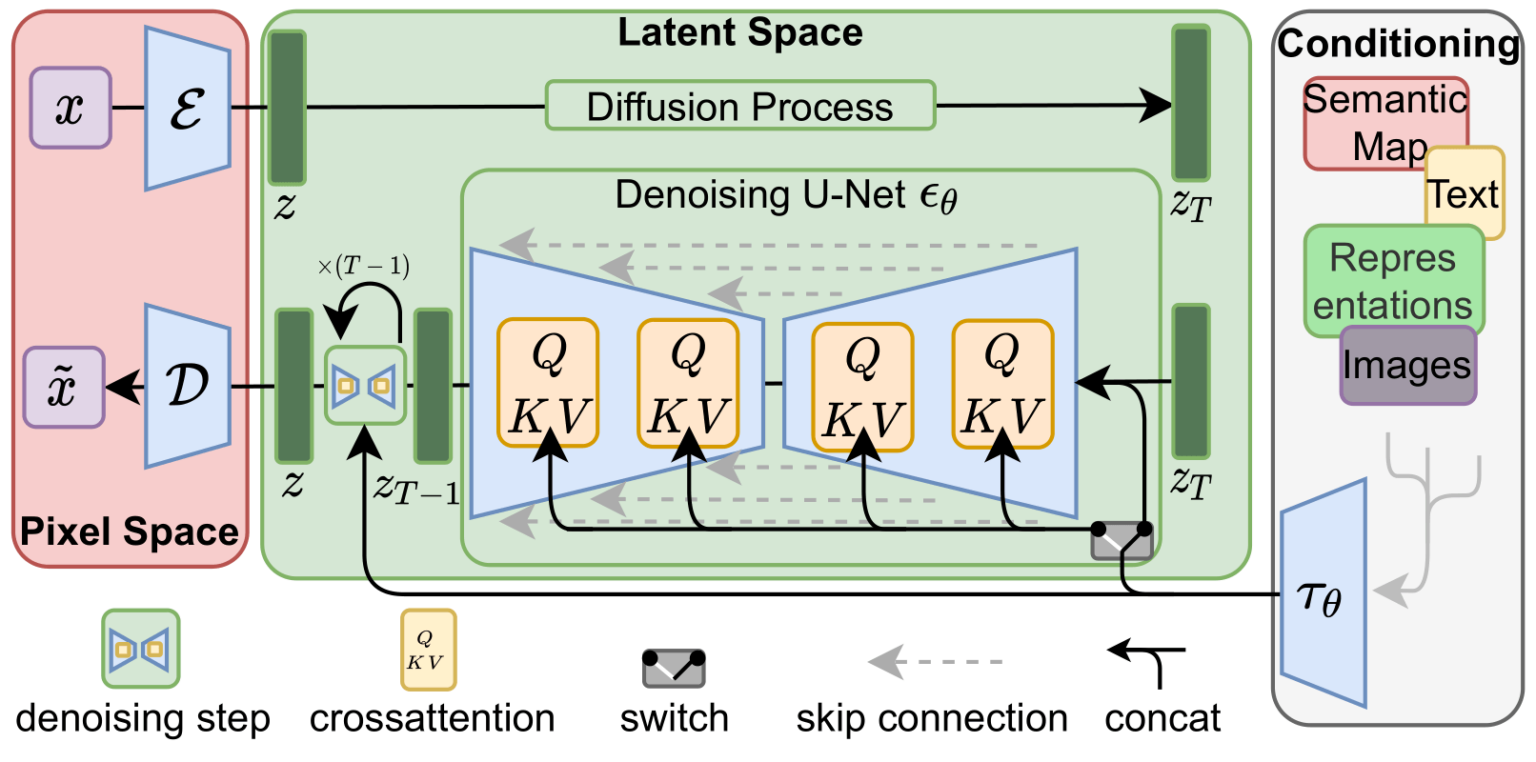
\includegraphics[width=\textwidth]{figures/2-sota/stable-diffusion.png}
    \caption[Stable diffusion architecture]{\textbf{Stable diffusion architecture} --- The Figure was taken from the original paper. On the top left, the original image $x$ is encoded with the \ac{AE}, and the diffusion process happens with the encodings. The text (or another data kind) is encoded with a transformer $\tau_{\theta}$, and these encodings are applied with attention to the denoising U-Nets. This denoising U-Net is applied $T$ times before the decoder transforms the encodings into an actual image in the pixel space again.}
    \label{fig:stable-diffusion}
\end{figure}
\subsubsection{Theoretical General Audio Transformer}

Transformers have become a prevalent architecture for several sequence modeling tasks in \ac{NLP}~\cite{gruetzemacher_deep_2022}. Their success has also expanded to the generative modeling of mediums such as images and videos. This section proposes adapting the transformer architecture for generative modeling and audio waveform synthesis.

A novel encoder-decoder transformer specifically designed for audio generation is introduced, referred to as the \acf{AT}. The \ac{AT} incorporates convolutional layers and custom attention mechanisms tailored to handle audio data.

The primary motivation is to enable high-quality, flexible audio generation for various applications. While transformers have proven effective in capturing long-range dependencies in sequences, the proposed \ac{AT} aims to optimize these models specifically for audio data.

The use of a transformer architecture for audio generation, propelled by textual prompts, is based on the encoder-decoder framework of the transformer, modified for audio synthesis. This configuration permits the effortless incorporation of textual data to aid in the synthesis of consistent and context-appropriate audio waveforms.

The process for generating audio using transformers includes two components: an encoder and a decoder. Each is composed of stacked layers that work together to process the textual input and create the corresponding audio output. The encoder's main function is to map the textual input to continuous representations that capture semantic information. For a deeper understanding on the encoder's functionality, as well as on transformers, in general, please refer to Section~\ref{sec:transformers}.

Upon receiving the continuous representations from the encoder, the decoder begins to generate the audio waveform. The decoder's functioning is dependent on the encoder's representations, which guarantees that the synthesized audio is aligned with the intended meaning of the input text. 

The synthesis process unfolds sequentially, with the decoder generating the output audio waveform sample-by-sample. The incorporation of multi-head attention mechanisms at the local and global levels enables the model to generate a wide range of natural-sounding audio outputs that correspond with the semantic context of the input.

The hyperparameters such as model dimensions, number of layers, attention heads, and hidden sizes can be tuned to balance performance and computational constraints. In summary, this architecture leverages the strengths of transformers for sequence modeling while optimizing the components for conditional audio generation.

\paragraph{Sound Representation}
Transformers have demonstrated power in autoregressive sequence modeling and generation. However, directly applying them to raw audio waveforms poses challenges due to the high sampling rates and lack of inherent discretization. As a potential alternative, spectrograms offer a 2D time-frequency audio representation (see section~\ref{sec:sound}). This section analyzes the trade-offs between raw audio versus spectrograms as inputs to transformer-based audio generation models.

\subparagraph{Challenges of Using Spectrograms}
Spectrograms explicitly encode frequency information, providing interpretable intermediate representations. However, transformers generate outputs one step at a time, and the notion of ``next'' becomes ambiguous on 2D spectrograms, as there are multiple values for each moment.

\subparagraph{Benefits of Raw Audio}
Raw audio waveforms allow direct modeling of the time-domain signal to be generated. The sequential structure matches the autoregressive nature of transformers without modification. Transformers can learn to model dependencies in the continuous waveform samples directly.
Raw audio represents the most natural fit for a sequential generation. Parameterizing waveform samples also avoids imposing and inverting a fixed spectrogram transformation that may discard information. Raw audio can capture nuances and exhibit fidelity beyond what prescribed spectrogram representations encode.

\subparagraph{Latent Feature Translation}
To fix these problems and bridge the gap between spectrograms and transformers, a novel approach is introduced. Instead of directly using the 2D spectrogram as input, a neural network is employed to translate each column of the spectrogram into a single continuous latent feature. This neural network, known from now on as the Latent Feature Translator, is shared across all columns and is conditioned on the corresponding timestamp of the column. The resulting continuous latent features capture the essential characteristics of the audio content while simplifying the representation for the subsequent transformer-based modeling.

This translation process effectively compresses the complex spectral information into a more manageable and informative format that still maintains temporal information, facilitating the transformer's ability to capture dependencies and generate coherent audio output.

This innovative approach leverages the strengths of both spectrogram representations and transformers, enabling efficient and effective generative audio modeling.

\paragraph{Training}

The \ac{AT} is first pretrained in an unsupervised manner to learn effective representations of audio data. During unsupervised pretraining, the model input is a segment of continuous latent features, and the target output is the next latent feature.

The model trains on audio-only data to predict the next latent feature. This relies on no text conditioning or labels. The goal is to learn generalized audio representations that capture dependencies across long sequences.

During training, audio clips are split into fixed-length chunks, 1-10 seconds. Batching multiple chunks together allows more efficient \ac{GPU} processing. Given all previous samples, the model is trained to predict the next latent feature at each step.

An error loss between the predicted and target audio samples is calculated. Over many training iterations, the model parameters are updated to minimize the loss function. Additional regularization techniques like dropout are used to prevent overfitting. The learning rate is gradually decayed for training as the loss function converges.

Validation audio clips not used in training monitor overfitting and determine early stopping. The model with the lowest validation loss is selected.

During supervised training, text conditioning is added to the pre-trained model. The loss function now optimizes conditional generation quality given input text.

This leverages the representations learned during unsupervised pretraining. Text conditioning trains the model to generate relevant audio for textual descriptions.

Pretraining provides an effective regularization technique to prime the model and prevent overfitting the paired text-audio data. This semi-supervised approach with unsupervised pretraining enables learning robust generative audio models.

\paragraph{Why Transformers}
Transformers are a natural choice for generative audio modeling compared to alternatives like \acp{GAN} or diffusion models (see Sections~\ref{sec:gan},~\ref{sec:diffusion}) due to their strength in sequential modeling. Audio signals inherently exhibit strong temporal consistency and context.

Transformers leverage a self-attention mechanism to model long-range dependencies in sequences effectively. This allows transformers to capture structures spanning longer time scales than recurrent models like \acp{LSTM} (see Section~\ref{sec:rnn-variants}). The global receptive field enables coherently modeling whole utterances, phrases, and even entire passages.

Additionally, as seen in Section~\ref{sec:transformers}, transformers have demonstrated state-of-the-art performance across various sequence transduction tasks in language, speech, and other domains. Leveraging their proven modeling capabilities for a new modality in audio is a natural progression.

The large model capacity of transformers is also advantageous, allowing sufficient expressivity to represent the complexity and nuance of audio data. With solid scalability to leverage large datasets through efficient parallel training, transformers are uniquely positioned as cutting-edge architecture for generative audio.

\paragraph{Limitations and Future Work}
While the \ac{AT} shows promise for generative audio modeling, there are several limitations and areas for improvement through future work.

First, the model requires large, diverse datasets of high-quality audio examples to train effectively. Collecting such datasets can be challenging, particularly for specialized domains like musical composition.

Data efficiency could be improved through transfer learning and unsupervised pretraining approaches. Leveraging models pretrained on other transformer tasks might provide valuable initializations for audio generation.

Training complex transformer models can also incur high computational costs and time requirements. Optimization for faster training and inference will be necessary for practical deployment. Architectural modifications to reduce model size should be explored.

Rigorously evaluating generated audio samples' coherence, naturalness, and creativity remains difficult. Developing quantitative and qualitative evaluation protocols to measure these attributes is an open research question.

There are many potential extensions to the base \ac{AT} architecture proposed here. For example, alternative conditioning mechanisms, sparser architectures optimized for audio, and adversarial training could improve results. Multi-task learning objectives that combine reconstruction, prediction, and discrimination may also help.

Multimodal integration of audio, text, and other modalities is also an exciting future direction. Jointly modeling text and audio could improve text-to-speech synthesis and transcription tasks. Exploring these multimodal representations with transformers is promising.

\paragraph{Innovative Approach}
Previous work has explored adapting transformers for raw audio generation, but these models have had limitations. Some, such as AudioGen~\ref{sec:audiogen}, have proposed transformer architectures for next-step audio sample prediction, demonstrating solid results for short-term modeling. However, these models do not allow conditional generation.

The proposed \ac{AT} builds on these predecessors to directly enable unconditional and conditional synthesis from the time-domain audio. By implementing an autoencoder, working on continuous latent features, and leveraging standard encoder-decoder transformers with pretraining, the \ac{AT} offers a novel approach to generative audio synthesis.

\subsection{Dataset Expansion}

Expanding the available datasets plays a critical role in training generative \ac{AI} models for audio synthesis. Larger and more diverse datasets provide models with a broader understanding of audio patterns, leading to more realistic and varied audio synthesis. In this subsection, we explore various strategies for dataset expansion, including the incorporation of new data augmentation techniques and the creation of new datasets through real-world recordings and crowdsourcing.

Data augmentation techniques are essential for increasing the diversity and size of the dataset. In the context of audio synthesis, several state-of-the-art data augmentation techniques have been proposed. These techniques can be seen in Section~\ref{sec:data-augmentation} and include time stretching, pitch shifting, noise injection, and others. By applying these techniques, one can artificially introduce variation into the dataset, allowing the models to learn from a wider range of audio patterns.

In future work, it is important to investigate the effectiveness of these data augmentation techniques in the context of audio synthesis. Specifically, the impact of each technique on the performance and generalization of generative models should be evaluated. This evaluation can be done by conducting systematic experiments that compare the performance of models trained with and without data augmentation. In addition, it would be valuable to investigate the combination of multiple data augmentation techniques to further increase the diversity and quality of the dataset.

Furthermore, the exploration of novel data augmentation techniques specifically tailored to audio data should be considered. This may involve exploring and adapting techniques from other domains, such as image or text data augmentation, and tailoring them to the unique characteristics of audio data. The development of domain-specific data augmentation techniques can potentially open up new possibilities for improving the realism and variety of audio synthesis.

Expanding the dataset may also involve creating new datasets that capture a broader range of audio characteristics. One approach is to include real-world recordings, such as live performances, field recordings, or professional studio recordings. These recordings provide a more realistic training environment for the models because they capture the nuances and complexities of real-world audio. Collaborating with musicians, audio engineers, or other experts in the field can ensure the acquisition of high-quality and diverse audio recordings.

Crowdsourcing provides an opportunity to expand the dataset by incorporating user-generated content from online platforms or social media. This approach allows for the inclusion of a diverse and constantly evolving dataset that reflects current trends and preferences in audio production. However, crowdsourced datasets come with their own challenges, such as ensuring data quality and addressing potential biases. Careful curation and validation processes should be implemented to maintain the integrity of the dataset.

\subsection{Evaluation Metrics}

Accurately evaluating the performance of generative \ac{AI} models' performance is challenging. Existing evaluation metrics often fail to capture the quality, variety, and realism of the generated audio. Future work should focus on developing robust evaluation metrics that align with human perception and subjective audio quality. By establishing reliable evaluation metrics, one can objectively evaluate and compare the performance of different models, facilitating advancements in the field.

As the dataset expands, it becomes necessary to develop new evaluation metrics that can assess the quality and diversity of the dataset. Existing evaluation metrics used in the field may have limitations in capturing the richness and diversity of the expanded datasets. Therefore, exploring and proposing new evaluation metrics that can effectively measure the performance and capabilities of generative models trained on the expanded datasets is important. These metrics should consider factors such as audio realism, diversity of generated outputs, and alignment with ground truth data.

By addressing these areas of future work, the scientific community can further advance the capabilities of generative \ac{AI} models for audio synthesis. Exploring novel architectures, expanding datasets, and developing improved evaluation metrics will contribute to the development of more powerful and reliable models, enabling applications in diverse domains such as music production, sound design, and interactive audio experiences.

\section{Conclusion} \label{sec:conc-conc}

In summary, this chapter has presented the conclusive results of an extensive investigation into the study and advancement of generative \ac{AI} models. The primary objectives of this research have been largely achieved, with the identification and discussion of the obstacles that prevented the full achievement of all objectives.

In addition, this study has significantly contributed to the existing body of knowledge on generative \ac{DL}. While developing end-to-end systems for sound synthesis from textual input remains arduous, particularly for researchers not affiliated with prominent technology companies, this thesis has made notable progress in this area. Initial prototypes have been developed, albeit with unsatisfactory results due to limitations in available datasets and the need for meticulous fine-tuning of hyper-parameters. Nevertheless, the potential for further improvement is recognized. Evaluating the ability of systems to generate sound from textual input also remains an ongoing challenge that warrants further investigation and refinement.

In conclusion, this research has provided invaluable insights into the study and development of generative \ac{AI}, focusing on audio synthesis. It has successfully achieved significant milestones, conducted a comprehensive investigation of \ac{DL} architectures and models, and made notable progress in creating end-to-end systems for sound synthesis.